%!TEX root = Main.tex




\subsection{End-to-end mobility case studies}
\label{sec:e2e}

\begin{figure*}[ht]
	\vspace{0.05in}
	\begin{minipage}[b]{0.48\linewidth}
		\centering
		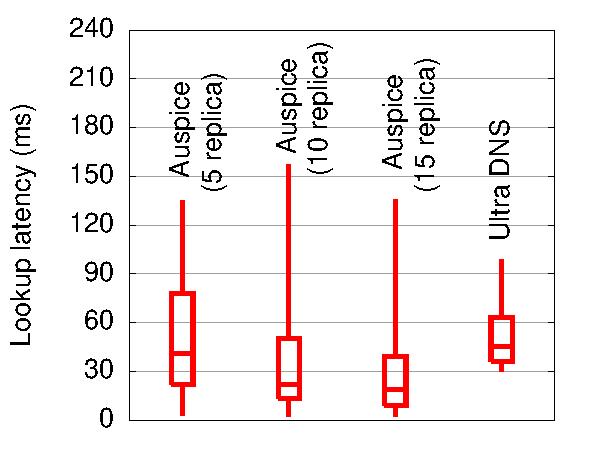
\includegraphics[width=2.8in,height=1.4in]{graph/newgraphs/managed-lookup.pdf}
		\figvsp
		\caption{Lookup latency:  \auspice\ with 5 replicas is comparable to UltraDNS (16 replicas); \auspice\ with 15 replicas has 60\% lower latency than UltraDNS.}
		\label{fig:managed-lookup}
	\end{minipage}
	\hspace{0.2in}
	\begin{minipage}[b]{0.48\linewidth}
		\centering
		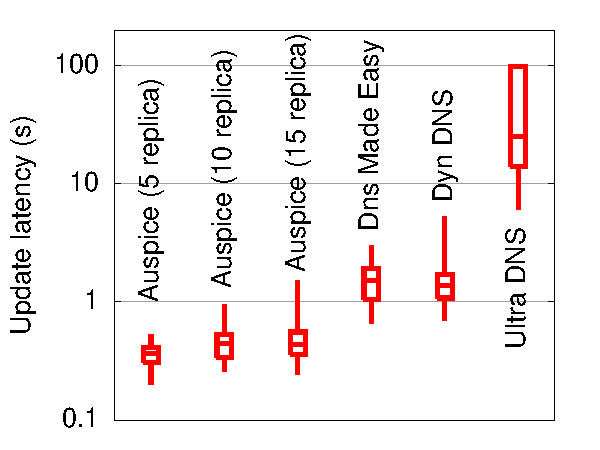
\includegraphics[width=2.8in,height=1.4in]{graph/newgraphs/managed-update.pdf}
		\figvsp
		\caption{Update propagation delay: \auspice\ with 5 replicas is  1.0 to 24.7 secs lower than three top-tier managed DNS service providers. }
		\label{fig:manageddnsupdate}
	\end{minipage}
	%\hspace{0.3cm}
	%\begin{minipage}[b]{0.3\linewidth}
	%\centering
	%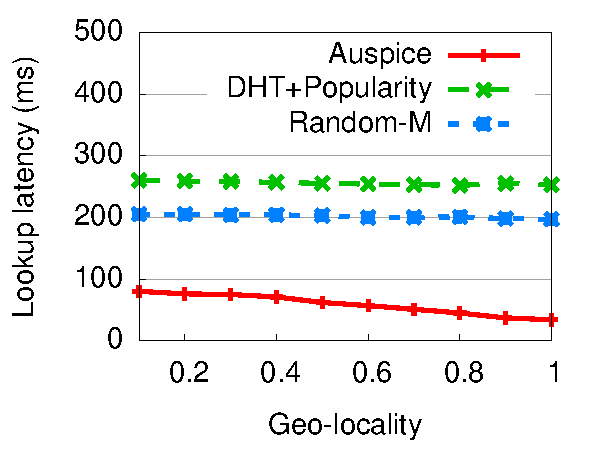
\includegraphics[width=2in,height=1.5in]{graph/medianlatencyVSlocality.pdf}
	%\figvsp
	%\caption{[Simulator] Workload sensitivity: \auspice\ lowers latency by 2--5$\times$  over \staticthree\ at all geo-locality levels.}
	%\label{fig:varylocality}
	%\end{minipage}
	\vspace{-0.25in}
\end{figure*}



Can \auspice\ serve as the basis of a complete end-to-end mobility solution? To address this question, we have developed \msocket, a user-level socket library that interoperates with \auspice, and supports all four types of endpoint mobility. %Using \auspice, \msocket\  supports connection migration, multipath communication, and mobile-to-mobile communication despite address-translating middleboxes using a distributed proxy service. 
The details of \msocket's design and implementation is the subject of a separate paper \cite{msocketTR}. Here, we {\em use} \msocket\ to show proof-of-concept of some of \auspice's capabilities.

\subsubsection{Time-to-connect to ``moving'' endpoints}
\label{sec:ttc_exp}

We evaluate the time-to-connect to a moving destination as a function of the mobility (or update) rate. The {\em end-to-end time-to-connect}  here is measured as the latency to look up an up-to-date address of the destination (or the time-to-connect as defined in Section \ref{sec:design_overview}) plus the time for msocket to successfully establish a TCP connection between the client and the mobile destination. This e2e-time-to-connect also incorporates the impact of timeouts and retried lookups if the client happens to have obtained a stale value (as in Fig. \ref{fig:4mobility}). The experiment is conducted on PlanetLab and consists of a single msocket client and a single mobile msocket server that is ``moving'' by changing its listening port number on a remote machine, and updating the name record replicated on three \auspice\ name servers accordingly. 
A successful connection setup delay using msocket is takes 2 RTTs (2 $\times$ 105 ms)  \cite{msocketTR}. 
As defined in Eq. \ref{eq:ttc}, the values of the update propagation latency $d_i$ and the lookup latency $l_i$ are 250 ms and 20 ms respectively, and the update rate $w_i$ varies from 1/1024/s to 1/s.
The timeout value ($T$) in our experiment is dependent on the RTT between the client and the server. If the client attempts to connect to the server on a port which the server is not listening on, the server immediately returns an error response to the client. Specifically, the timeout value is either 1 or 2 RTTs with equal probability depending on whether the connection failed during the first or the second round-trip of msocket's connection setup.
The client sends lookups at a rate of 10/s (but this rate does not affect the time-to-connect), and both lookups and updates inter-arrival times are exponentially distributed.


Figure \ref{fig:ttc_msocket} shows the distribution of the time-to-connect with update propagation delays entailed by eventual consistency. For low-to-moderate mobility rates ($<\frac{1}{64s}$), we find that all time-to-connect values are close to 230 ms, of which 20ms is the lookup latency, and 210ms is msocket's connection setup latency. The reason the client is able to obtain the correct value upon first lookup in all cases is that the update propagation latency of 250ms is much smaller than the average inter-update interval (64s).  The update propagation delay becomes a non-trivial fraction of the inter-update interval at high mobility rates of $\approx$1/sec that results in  26\% of lookups returning stale values. The mean e2e-time-to-connect increases to  302 ms for an update rate of 1/sec, which suggests that \auspice's time-to-connect is limited by network propagation delays in this regime. Nevertheless, once a connection is successfully established, {individual} migration can quickly resynchronize the connection in $\approx$two round-trips between the client and the mobile without relying on \auspice\ (not shown here). 
%A different experiment with totally ordered writes shows qualitatively similar conclusions \cite{techreport}.

Figure \ref{fig:ttc_msocket} also shows that the time-to-connect as predicted by our analytical model (Eq. \ref{eq:ttc}) are close to those observed in the experiment, thereby re-affirming our design. 

%\blue{We evaluate the time-to-connect to a moving destination as a function of the mobility (or update) rate. We stick with the running definition of time-to-connect used in the paper, namely, the time to look up an up-to-date address of the destination, i.e., an address to which the client can successfully establish a TCP connection. This definition excludes the (successful) connection setup delay itself as that delay is independent of \auspice's design, but it does incorporate the impact of timeouts and retried lookups if the client happens to have obtained a stale value (as in Fig. \ref{fig:4mobility}). The experiment is conducted on PlanetLab and consists of a single virtual client and a single virtual mobile server that is ``moving'' by changing its listening port number on a remote machine, and updating the name record replicated on three \auspice\ name servers accordingly. As defined in Eq. \ref{eq:ttc}, the values of the timeout $T_i$ and lookup latency $l_i$ are 5 secs and 50 ms respectively, and the update rate $w_i$ varies from $10^{-4}$/s to 1/s. The client sends lookups at a rate of 10/s (but this rate does not affect the time-to-connect), and both lookup and update inter-arrival times are exponentially distributed}

%\blue{Figure \ref{fig:ttc} shows the distribution of the time-to-connect with update propagation delays entailed by eventual consistency. For low-to-moderate mobility rates ($< 0.01/$s), we find that all lookup latencies are much smaller than 5 sec and mean time-to-connect is less than 50 ms, i.e.,  the client is able to obtain the correct value upon first lookup in all cases. This is because the update propagation latency of 190 ms is much smaller than the average inter-update interval (100 s).  The update propagation delay becomes a non-trivial fraction of the inter-update interval at high mobility rates of 0.1 to 1/sec that respectively result in 1.5\% and 13\% of timeouts for lookups. The mean time-to-connect increases to  641 ms for an update rate of 1/sec, which suggests that \auspice's time-to-connect is limited by network propagation delays in this regime. Nevertheless, once a connection is successfully established, {individual} migration can quickly resynchronize the connection in about two round-trips between the client and the mobile without relying on \auspice\ (not shown here). %A different experiment with totally ordered writes shows qualitatively similar conclusions \cite{techreport}.}

%\blue{Figure \ref{fig:ttc} also shows that the time-to-connect as predicted by our analytical model (Eq. \ref{eq:ttc}) is close to those observed in the experiment, thereby re-affirming our design. }

\eat {
	% sequential single-column figures
	
	\begin{figure}[ht]
		\vsp
		\centering
		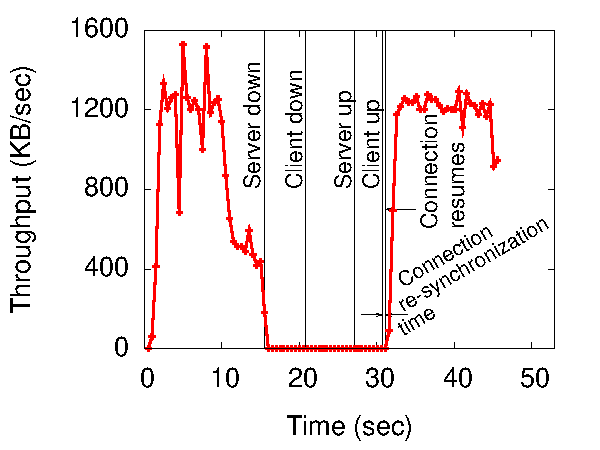
\includegraphics[width=3in, height=1.5in]{figure/SimulMig.pdf}
		\figvsp
		\caption{Simultaneous mobility recovery in $\approx$2 RTTs after both endpoints resurface.}
		\label{fig:SimulMig}
	\end{figure}
	
	\begin{figure}[ht]
		\figvsp
		\centering
		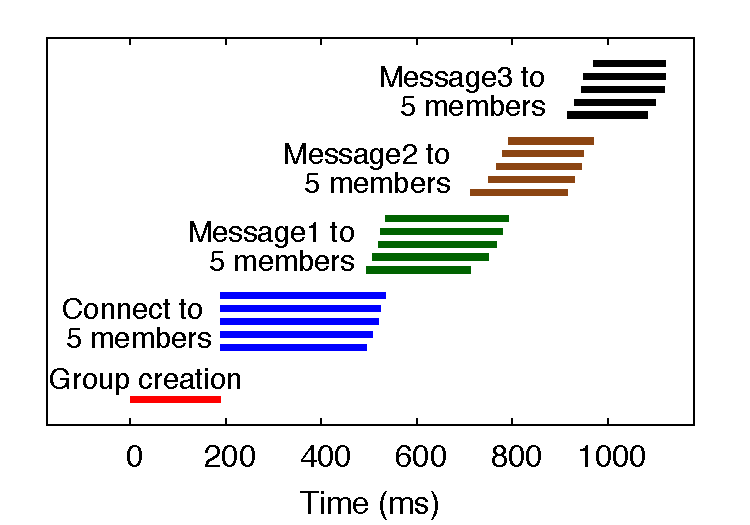
\includegraphics[width=2in, height=1.5in]{figure/5MemTimeLineUsed.pdf}
		\figvsp
		\caption{Context-aware delivery timeline showing 3 messages being geo-cast to 5 members.}
		\label{fig:5MemberTimeline}
		\figvsp
	\end{figure}
}





\subsubsection{Simultaneous endpoint mobility}

Figure \ref{fig:SimulMig} shows an experiment involving simultaneous mobility. The client is an Android phone using \msocket\ via a WiFi interface to connect to a publicly addressable Planetlab machine at time 0. The server and client shut down their interfaces respectively around 15 and 20 sec. Subsequently, the server restarts its interface and starts listening on a different port and updates \auspice\ accordingly. After that, the client restarts its interface and attempts to re-synchronize the connection. This re-synchronization time is roughly 300ms as shown and consists of the following delays. The client performs a query to \auspice\ to resolve the server's GUID to its new socket address (IP, port), which takes roughly 50ms and mostly corresponds to the round-trip delay between the client and the \auspice\ nameserver. The remaining 250ms roughly correspond to 2 RTTs of delay between the client and the server that are separated by a round-trip delay of 120ms.

\subsubsection{Context-aware delivery}
\label{sec:context}

Next, we show a proof of concept of context-aware communication, a novel communication primitive enabled by \auspice's extensible key-value API. \auspice\ allows applications to bind an \msocket\ not only to human-readable names or GUIDs, but also to abstract context descriptors as in \verb+msocket.bind("[geoloc: [lat,long],radius]")+.  Writes to this \msocket\ are reliably delivered to all GUIDs in the geo-fence created by this descriptor. Underneath the covers, \msocket\ invokes \auspice\ to create on-demand a {group GUID}, i.e., a  GUID with a membership field consisting of a set of member GUIDs, and obtains this member set. \msocket\ internally resolves each member GUID to its socket address and establishes an \msocket\ connection for reliably delivery.

Figure \ref{fig:5MemberTimeline} shows an experiment involving a group creator (also the message sender) on an Android phone and a number of potential members on PlanetLab nodes, 5 of which fake-register their coordinates in \auspice\ so as to appear to be within the created geo-fence. The RTT between the group creator and members is 125ms. The figure shows that group creation, a single call to \auspice\ that returns all member GUIDs, takes roughly 200ms. Subsequently, an internal \msocket\ connect to each member involves another \auspice\ lookup to resolve the GUID to a socket address and connect in parallel to all 5 members, which takes 250-280ms. After this, the creator sends 3 short messages back-to-back that each take roughly 1 RTT to be reliably delivered.

%Context-aware group GUIDs in \auspice\ are active, i.e., \auspice\ refreshes the membership set periodically so that if an existing member leaves or a new member arrives into the context-space, the group GUID is updated accordingly. This refresh interval limits how responsive context-aware communication is to member churn. 
More details of optimizing context-aware queries in \auspice, reducing membership staleness, the connection migration protocol, etc. are outside the scope of this paper \cite{msocketTR}. This experiment seeks only to exemplify a powerful, new communication primitive enabled by context descriptors compared to strictly hierarchical DNS names, as argued in Section \ref{sec:whyNotDNS}. 














